\chapter{Systembeschreibung}

Das nachfolgende Kapitel befasst sich mit der Beschreibung der Technologien und Vorgehensweisen, die zur Link Discovery im Rahmen dieser Arbeit angewendet wurden. Dazu zählen im Einzelnen die gewählte Datenbank MongoDB, das Datenmodell des Zielgraphen und das daraus resultierende Vorgehen und die Architektur des Systems zur Link Discovery.

\section{MongoDB}

\section{Datenmodell}

\begin{figure}
\label{fig:graph_model}
\begin{center}
    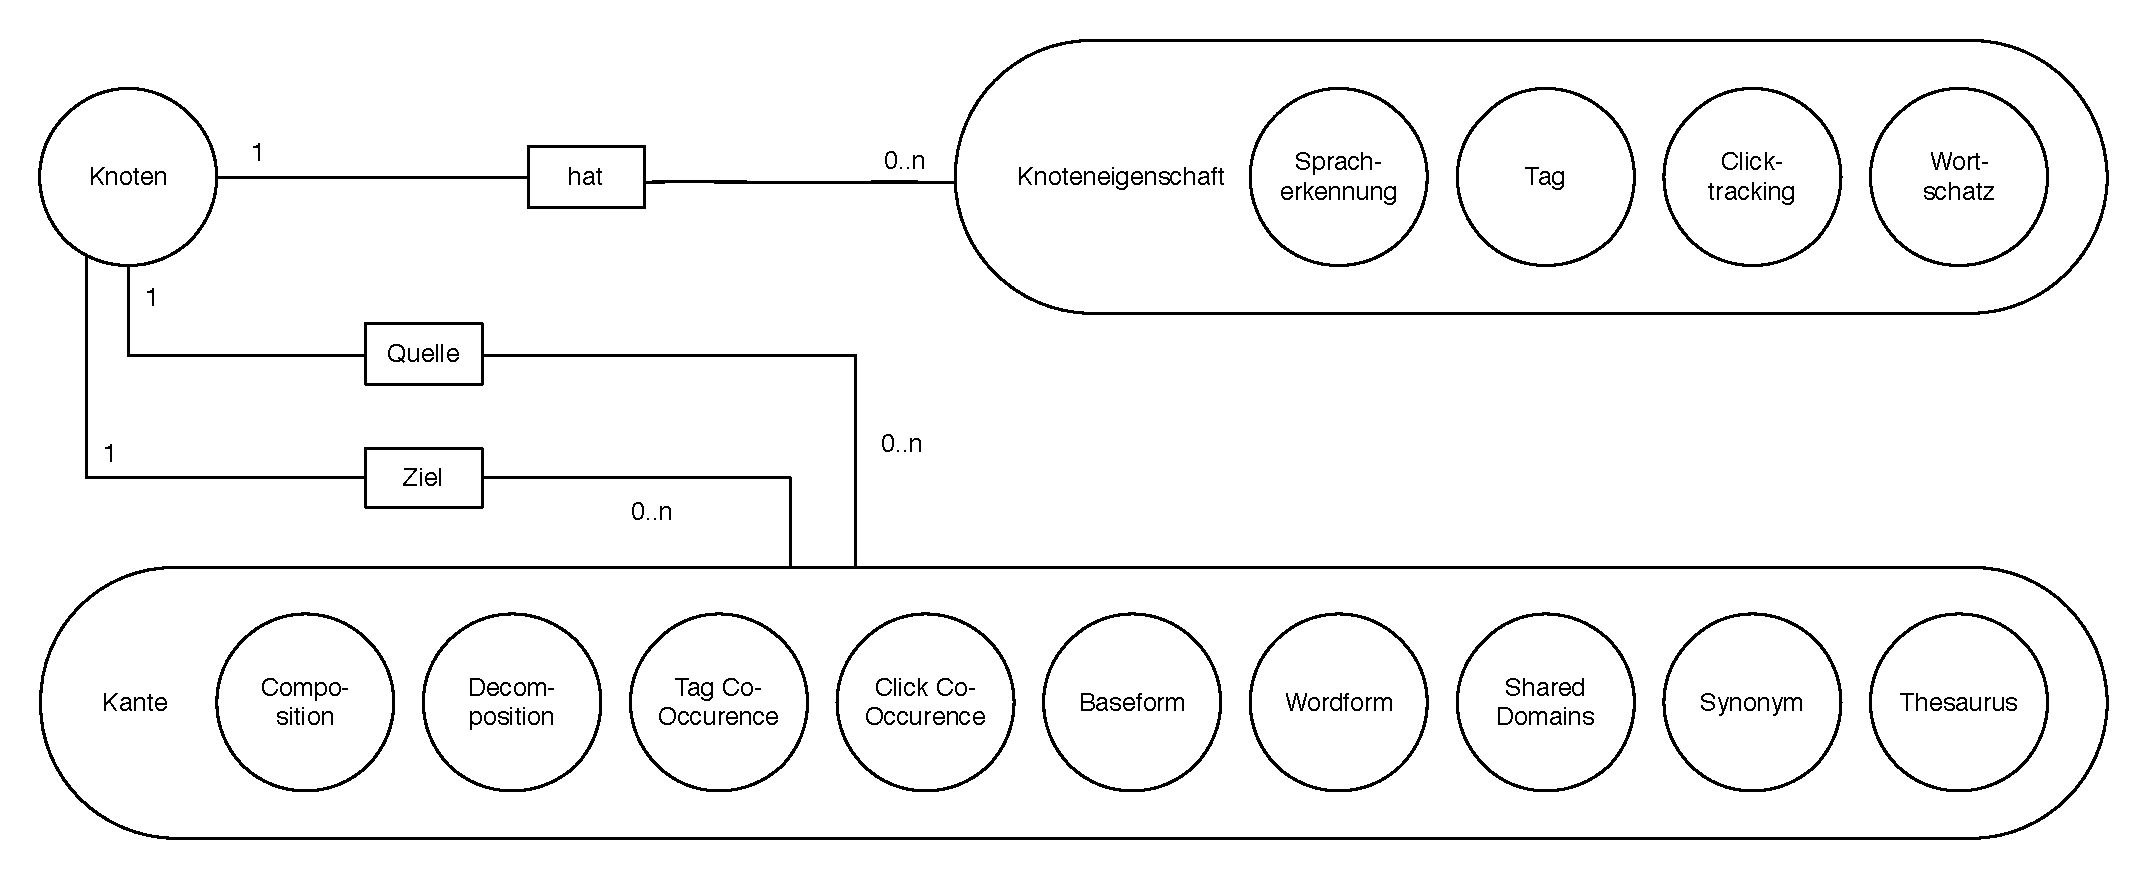
\includegraphics[width=1\textwidth]{graph_model}
\end{center}
\caption{Datenmodell des Graphen als Entity-Relationship-Diagramm}
\end{figure}

\section{Systemarchitektur}

\begin{figure}
\label{fig:architecture}
\begin{center}
    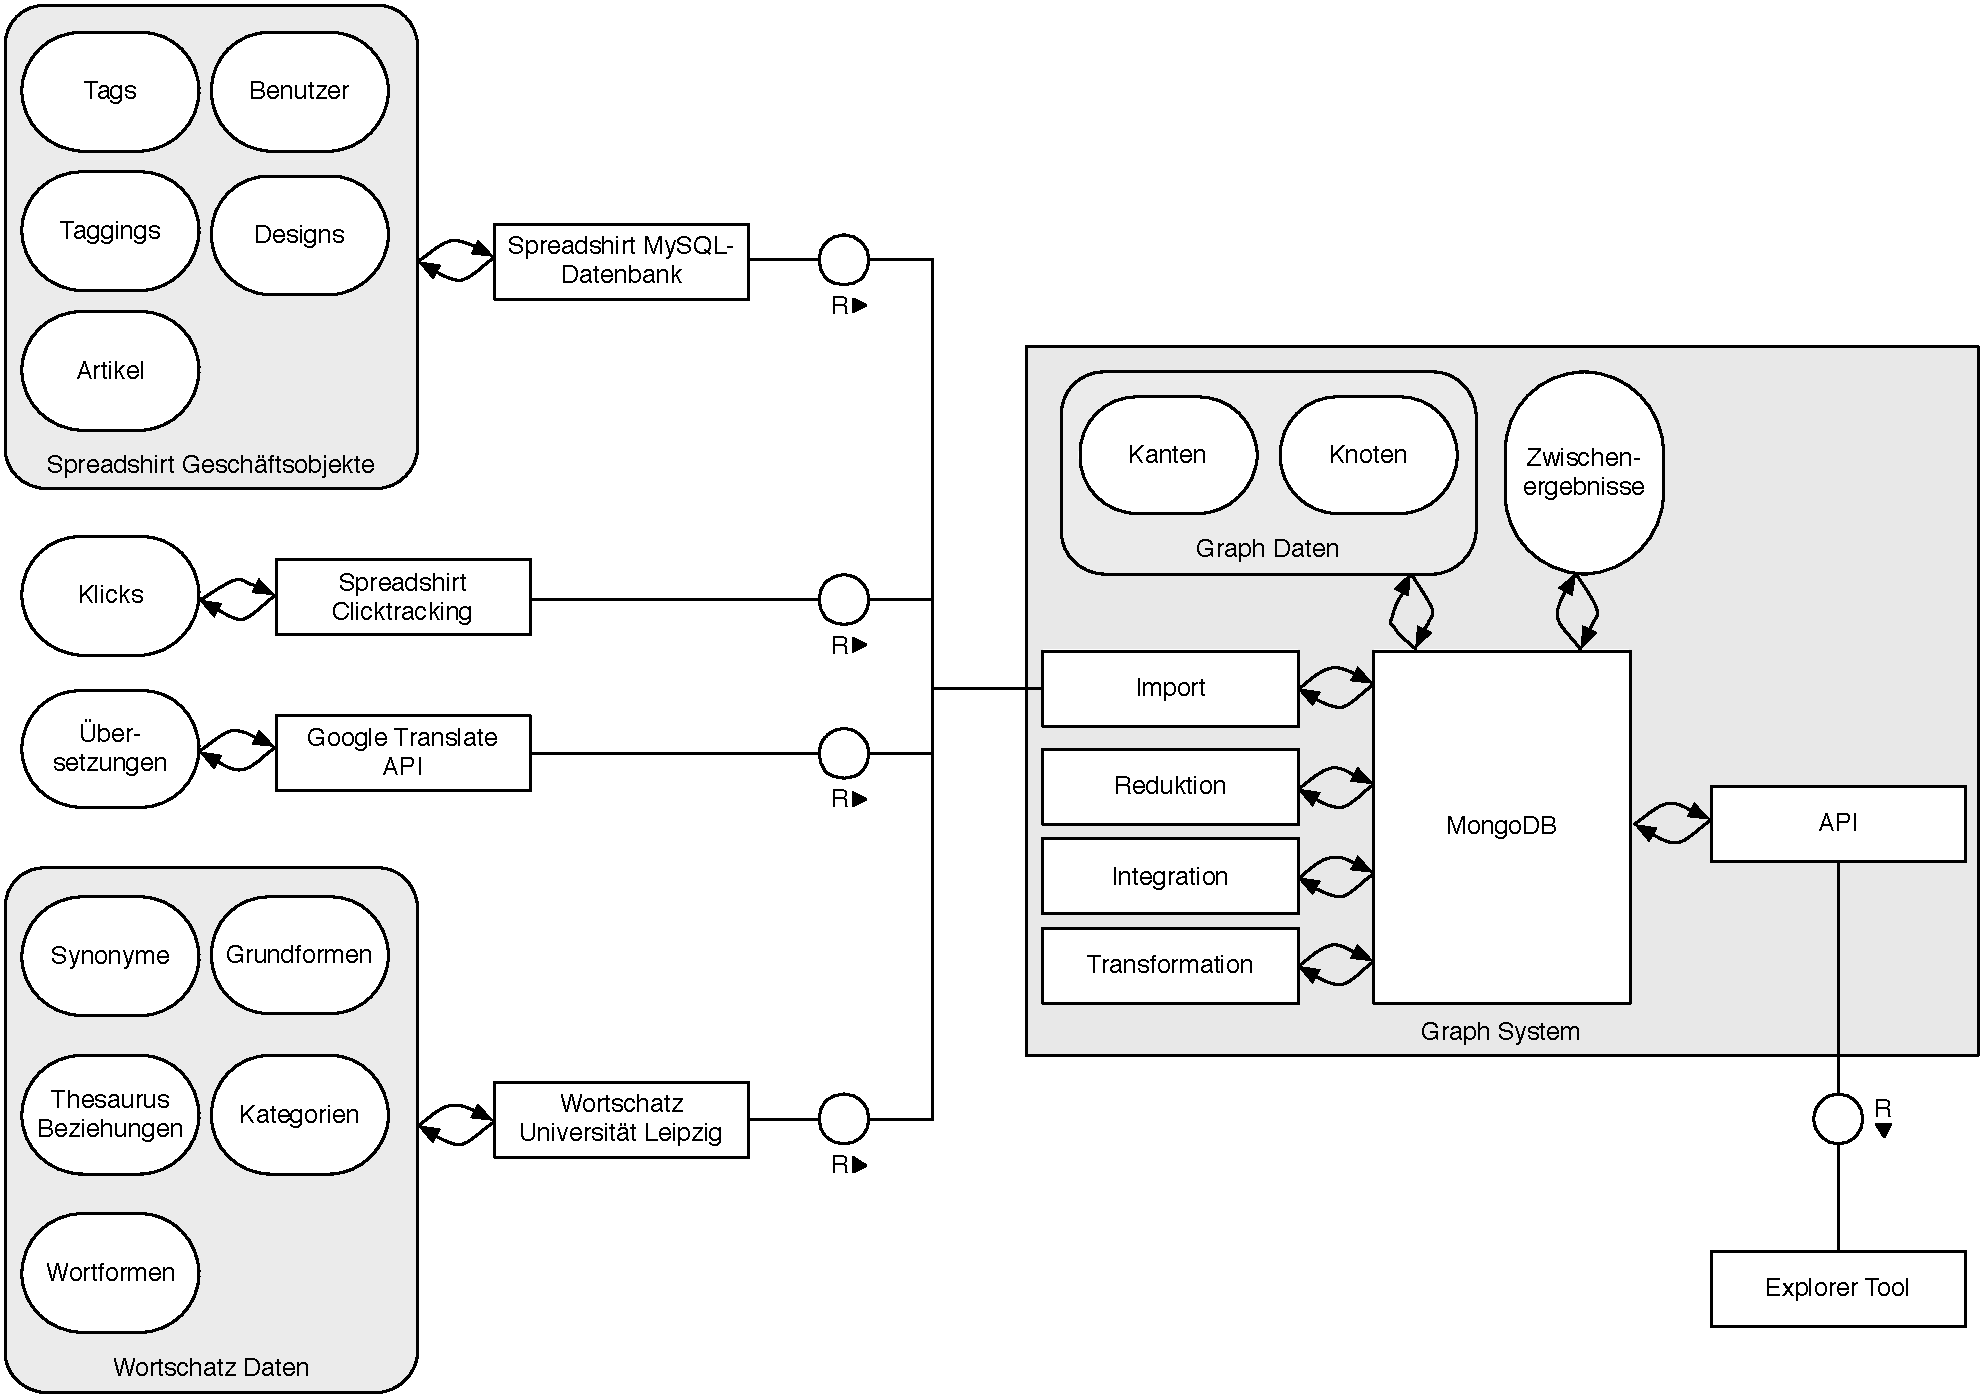
\includegraphics[width=1\textwidth]{architecture}
\end{center}
\caption{Systemarchitektur}
\end{figure}
